\section{The Regionalized Value State Dependence Graph}\label{sec:rvsdg}
A Regionalized Value State Dependence Graph (RVSDG) is an acyclic hierarchical multigraph
consisting of nested regions. A region $\Region = (A, N, E, R)$ represents a computation with
argument tuple $A$, nodes $N$, edges $E$, and result tuple $R$, as illustrated
in Figure~\ref{fig:notation}. A node can be either
\emph{simple}, \ie, it represents a primitive operation, or \emph{structural}, \ie, it
contains regions. Each node $\n \in N$ has a tuple of inputs $I$ and outputs $O$. In case of
simple nodes, they correspond to arguments and results of the represented operation, whereas for
structural nodes, they map to arguments and results of the contained regions. For nodes
$\node{}{1}, \node{}{2} \in N$, an edge $\edgeb{\org}{\usr} \in E$ connects either output
$\org \in O_{n_1}$ or argument $\org \in A$ to either input $\usr \in I_{n_2}$ or result
$\usr \in R$ of matching type. We refer to \org as the \emph{origin} of an edge, and to \usr as the
\emph{user} of an edge. Every input or result is the user of \emph{exactly one} edge, whereas
outputs or arguments can be the origins of multiple edges. All inputs or results of an origin are
called its \emph{users}. The corresponding node of an origin is called its \emph{producer}, whereas
the corresponding node of a user is called \emph{consumer}. Correspondingly, the set of nodes of
all users of an origin are referred to as its \emph{consumers}. The types of inputs and outputs
are either \emph{values}, representing arguments or results of computations, or \emph{states}, used
to impose an order on operations with side-effects. A node's \emph{signature} are the
types of its inputs and outputs, whereas a region's signature are the types of its arguments
and results. %
Throughout this paper, we use \n, \e, \ipt, \opt, \argmnt, and \res with
sub- and superscripts to denote individual \textbf{n}odes, \textbf{e}dges, \textbf{i}nputs,
\textbf{o}utputs, \textbf{a}rguments, and \textbf{r}esults, respectively. We use \org and \usr to
denote an edge's ori\textbf{g}in and \textbf{u}ser, respectively. An edge \e from origin \org to
user \usr is also denoted as \edgec{\e}{\org}{\usr}, or short \edgeb{\org}{\usr}.

The RVSDG can model programs at different abstraction levels. It can represent simple
data-flow graphs such as those used in machine learning frameworks, but it can also represent
programs at the machine level as used in compiler back-ends for code generation. This
flexibility makes it possible to use the RVSDG for the entire compilation pipeline. In this paper,
we target an abstraction level similar to that of LLVM IR. This permits us to illustrate all of
the RVSDG's features without involving architecture-specific details. The rest of this section
defines the necessary constructs.

\subsection{Intra-procedural Nodes}\label{sec:intra-nodes}

This section defines the nodes for representing the intra-procedural aspects of programs. It
explains simple nodes and discusses the two structural nodes required for modeling intra-procedural
program behavior:

\begin{enumerate}
	\item \emph{Gamma-Nodes} model conditionals with symmetric split and joins, such as
		\texttt{if-then-else} statements.
	\item \emph{Theta-Nodes} represent tail-controlled loops, \ie, \texttt{do-while} loops.
\end{enumerate}

\subsubsection{Simple nodes}
Simple nodes model primitive operations such as addition, subtraction, load, and store. They have
an operator associated with them, and a node's signature must correspond to the signature of
its operator. Simple nodes map their input value tuple to their output value tuple by evaluating
their operator with the inputs as arguments, and associating the results with their outputs.
Figure \ref{fig:expr} illustrates the use of simple nodes as well as value and state edges. Solid
lines represent value edges, whereas dashed lines represent state edges. Nodes have as many
value inputs and outputs as their corresponding operations demand. The ordering of the load and
store nodes is preserved by sequentializing them with the help of state edges.

\begin{figure*}
	\subfloat[Notation\label{fig:notation}]{
			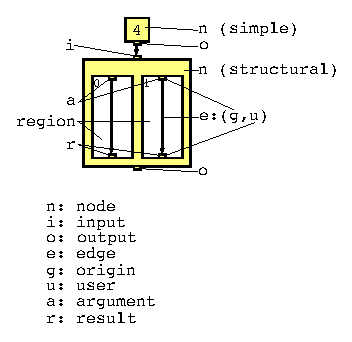
\includegraphics[scale=0.84]{notation-updated}
	}
	\hfill
	\subfloat[Simple nodes\label{fig:expr}]{
			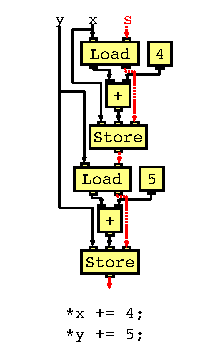
\includegraphics[scale=0.84]{simple_nodes}
	}
	\hfill
	\subfloat[\gammanode\label{fig:gamma}]{
			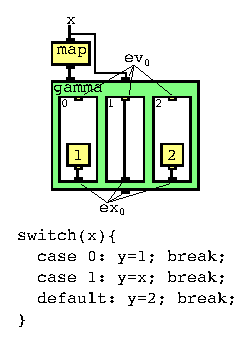
\includegraphics[scale=0.84]{gamma}
	}
	\hfill
	\subfloat[\thetanode\label{fig:theta}]{
			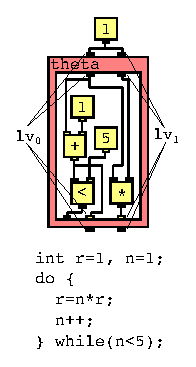
\includegraphics[scale=0.84]{theta}
	}
	\caption{Notation as well as examples for the usage of simple, \gammam and \thetanodes.}
	\label{fig:example}
\end{figure*}

\subsubsection{Gamma-Nodes}
A \gammanode models a decision point and contains regions
$\Region_0, ..., \Region_k \mid k > 0$ of matching signature. Its first input is a
\emph{predicate}, which determines the region under evaluation. It evaluates to an
integer $v$ with $0 \le v \le k$. The values of all other inputs are mapped to the corresponding
arguments of region $\Region_v$, $\Region_v$ is evaluated, and the values of its results are mapped
to the outputs of the \gammanode.

\gammanodes represent conditionals with symmetric control flow splits and
joins, such as \verb;if-then-else; or \verb;switch; statements without fall-throughs. Figure
\ref{fig:gamma} shows a \gammanode. It contains three regions: one for each case, and a default
region. The map node takes the value of $x$ as input and maps it to zero, one, or two, determining
the region under evaluation. This region is evaluated and its result is mapped
to the \gammanode's output.

We define the \emph{entry variable} of a \gammanode as a pair of an input and the arguments the
input maps to during evaluation, as well as the \emph{exit variable} of a \gammanode as a pair of
an output and the results the output could receive its value from:

\begin{definition}
The pair $ev_{l} = (\iput{}{l+1}, A_{l})$ is the $l$-th \emph{entry variable} of a \gammanode with
$k+1$ regions. It consists of the $l+1$-th input and tuple $A_{l} = \{a^{\Region_0}_{l}, ...,
a^{\Region_k}_{l}\}$ with the $l$-th argument from each region. We refer to the set of all
entry variables as $EV$.
\end{definition}

\begin{definition}
The pair $ex_{l} = (R_l, \oput{}{l})$ is the $l$-th \emph{exit variable} of a \gammanode with $k+1$
regions. It consists of a tuple $R_l = \{r^{\Region_0}_l, ...,r^{\Region_k}_l\}$ of the $l$-th
result from each region and the $l$-th output they would map to. We refer to the set of all exit
variables as $EX$.
\end{definition}

Figure~\ref{fig:gamma} shows the \gammanode's only entry and exit variable annotated.

\subsubsection{Theta-Nodes}
A \thetanode models a tail-controlled loop. It contains one
region that represents the loop body. The length and signature of its input tuple equals that of
its output, or the region's argument tuple. The first region result is a \emph{predicate}.
Its value determines the continuation of the loop. When a \thetanode is evaluated, the values of
all its inputs are mapped to the corresponding region arguments and the body is evaluated. When
the predicate is true, all other results are mapped to the corresponding arguments for the next
iteration. Otherwise, the result values are mapped to the corresponding outputs. The loop
body of an iteration is always fully evaluated before the evaluation of the next iteration.
This avoids ``deadlock`` problems between computations of the loop body and the predicate, and
results in well-defined behavior for non-terminating loops that update external state.

\thetanodes permit the representation of \verb;do-while; loops. In combination with \gammanodes,
it is possible to model head-controlled loops, \ie, \verb;for; and \verb;while; loops. Thus,
employing tail-controlled loops as basic loop construct enables us to express more complex loops as
a combination of basic constructs. This normalizes the representation and reduces the complexity
of optimizations as there exists only one construct for loops. Another benefit of tail-controlled
loops is that their body is guaranteed to execute at least once, enabling the unconditional
hoisting of invariant code with side-effects.

Figure \ref{fig:theta} shows a \thetanode with two loop variables, $n$ and $r$, and an additional
result for the predicate. When the predicate evaluates to true, the results for $n$ and
$r$ of the current iteration are mapped to the region arguments to continue with the next
iteration. When the predicate evaluates to false, the loop exits and the results are mapped to the
node's outputs. We define a \emph{loop variable} as a quadruple that represents a value routed
through a \thetanode:

\begin{definition}
The quadruple $lv_{l} = (\iput{}{l}, \argument{}{l}, \result{}{l+1}, \oput{}{l})$ is the $l$-th
\emph{loop variable} of a \thetanode. It consists of the $l$-th input \iput{}{l}, argument
\argument{}{l}, and output \oput{}{l}, and the $l+1$-th result of a \thetanode. We refer to
the set of all loop variables as $LV$.
\end{definition}

Figure~\ref{fig:theta} shows the \thetanode's two loop variables annotated.

\subsection{Inter-procedural Nodes}\label{sec:inter-nodes}
This section defines the four structural nodes used for modeling the inter-procedural aspects of
programs:

\begin{enumerate}
	\item \emph{Lambda-Nodes} are used for modeling procedures and functions.
	\item \emph{Delta-Nodes} model global variables.
	\item \emph{Phi-Nodes} represent mutually recursive environments, such as (mutually) recursive
		functions.
	\item \emph{Omega-Nodes} represent translation units.
\end{enumerate}

\subsubsection{Lambda-Nodes}
A \lambdanode models a function and contains a single region representing a
function's body. It features a tuple of inputs and a single output. The inputs refer to external
variables the \lambdanode depends on, and the output represents the \lambdanode itself. The region
has a tuple of arguments comprised of a function's external dependencies and its arguments, and a
tuple of results corresponding to a function's results.

An \applynode represents a function invocation. Its first input takes a \lambdanode's output
as origin, and all other inputs represent the function arguments. In the rest of the paper, we
refer to an \applynode's first input as its \emph{function input}, and to all its other inputs as
its \emph{argument inputs}. Invocation maps the values of a $\lambda$-node's input $k$-tuple to the
first $k$ arguments of the \lambdaregion, and the values of the function arguments of the
\applynode to the rest of the arguments of the \lambdaregion. The function body is evaluated and
the values of the \lambdaregion's results are mapped to the outputs of the \applynode.

Figure \ref{fig:lambda} shows an RVSDG with two \lambdanodes. Function $f$ calls functions $puts$
and $max$ with the help of \applynodes. The function $max$ is part of the translation unit, while
$puts$ is external and must be imported (see the paragraph about \omeganodes for more details).
We further define the \emph{context variable} of a \lambdanode. A context variable provides the
corresponding input and argument for a variable a \lambdanode depends on.

\begin{figure*}
	\subfloat[RVSDG with \lambdam and \deltanodes\label{fig:lambda}]{
		\begin{minipage}{0.5\textwidth}
			\centering
			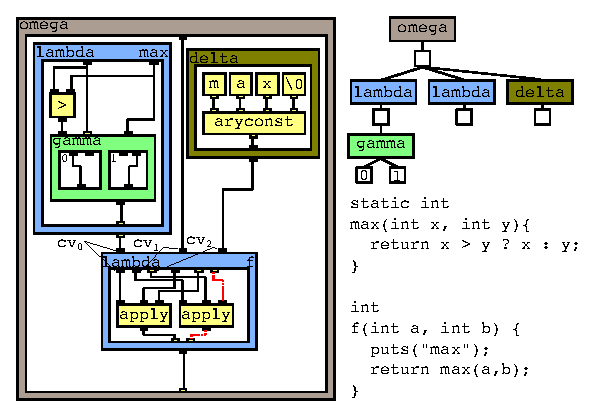
\includegraphics[scale=0.82, valign=c]{lambda}
			\vphantom{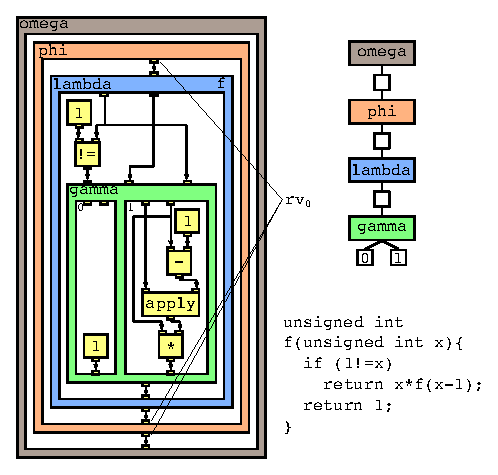
\includegraphics[scale=0.82, valign=c]{phi}}
		\end{minipage}
	}
	\subfloat[RVSDG with a \phinode\label{fig:phi}]{
		\begin{minipage}{0.5\textwidth}
			\centering
			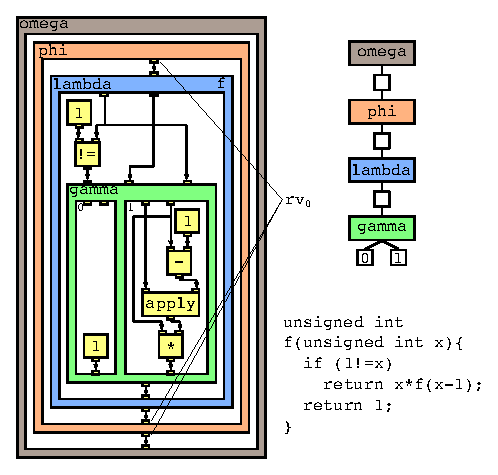
\includegraphics[scale=0.82, valign=c]{phi}
		\end{minipage}
	}
	\caption{Example for the usage of \lambdam, \deltam, and \phinodes, as well as corresponding
		region trees.}
	\label{fig:example2}
\end{figure*}

\begin{definition}
The pair $cv_{l} = (\iput{}{l}, \argument{}{l})$ is a \lambdanode's $l$-th \emph{context variable}.
It consists of the $l$-th input and argument. We refer to the set of all context
variables as $CV$.
\end{definition}

Figure~\ref{fig:lambda} shows the three context variables of fuction $f$ annotated: one for
function $max$, one for function $puts$, and one for the global variable representing the string
argument to $puts$.

\begin{definition}
The \lambdanode connected to a function input is the \emph{callee} of an \applynode, and an
\applynode is the \emph{caller} of a \lambdanode. We refer to the set of all callers of a
\lambdanode as $CLL$.
\end{definition}

\subsubsection{Delta-Nodes}
A \deltanode models a global variable and contains a single region representing the constants'
value. It features a tuple of inputs and a single output. The inputs refer to the external
variables the \deltanode depends on, and the output represents the \deltanode itself. The region
has a tuple of arguments representing a global variable's external dependencies and a single
result corresponding to its right-hand side value.

Figure~\ref{fig:lambda} shows an RVSGD with a \deltanode. Function $puts$ takes a string as
argument that is the right-hand side of a global variable.
Similarly to \lambdanodes, we define the \emph{context variable} of a \deltanode. It provides the
corresponding input and argument for a variable a \deltanode depends on.

\begin{definition}
The pair $cv_{l} = (\iput{}{l}, \argument{}{l})$ is a \deltanode's $l$-th \emph{context variable}.
It consists of the $l$-th input and argument. We refer to the set of all context variables as $CV$.
\end{definition}

\subsubsection{Phi-Nodes}
A \phinode models an environment with mutually recursive functions, and contains
a single region with \lambdanodes. Each single output of these \lambdanodes serves as origin to a
single result in the \phiregion. A \phinode's outputs expose the individual functions to callers
outside the \phiregion, and must therefore have the same arity and signature as the results of the
\phiregion. The first input of an \applynode from \emph{outside} the \phiregion takes these
outputs as origin to invoke one of the functions.

The inputs of a \phinode refer to variables that the contained functions depend on and are mapped
to corresponding arguments in the \phiregion when a function is invoked. In addition, a
\phiregion has arguments for each contained function. An \applynode from
inside a \phiregion takes these as origin to its function input.

\phinodes permit a program's mutually recursive functions to be expressed in the RVSDG
without the introduction of cycles. Figure \ref{fig:phi} shows an RVSDG with a \phinode.
The function $f$ calls itself, and therefore needs to be in a \phinode to preserve the RVSDG's
acyclicity. The region in the \phinode has one input, representing the declaration of $f$, and
one output, representing the definition of $f$. The \phinode has one output so that $f$ can
be called from outside the recursive environment.

We define \emph{context variables} and \emph{recursion variables}. Context variables
provide corresponding inputs and arguments for variables the \lambdanodes from within a \phiregion
depend on. Recursion variables provide the argument and output an \applynode's function
input connects to.

\begin{definition}
The pair $cv_{l} = (\iput{}{l}, \argument{}{l})$ is the $l$-th \emph{context variable} of a
\phinode. It consists of the $l$-th input and argument. We call the set of all context variables
$CV$.
\end{definition}

\begin{definition}
For a \phinode with $n$ context variables, the triple $rv_{l} = (\result{}{l}, \argument{}{l+n},
\oput{}{l})$ is the $l$-th \emph{recursion variable}. It consists of the $l$-th result and
$l+n$-th argument of the \phiregion as well as the $l$-th output of the \phinode. We refer to the
set of all recursion variables as $RV$.
\end{definition}

Figure~\ref{fig:phi} shows the the \phinode's recursion variable annotated.

\subsubsection{Omega-Nodes}
An \omeganode models a translation unit. It is the top-level node of an
RVSDG and has no inputs or outputs. It contains exactly one region. This region's
arguments represent entities that are external to the translation unit and therefore need to be
imported. Its results mark all exported entities in the translation unit. Figure
\ref{fig:lambda} and \ref{fig:phi} illustrate the usage of \omeganodes. The \omegaregion in Figure
\ref{fig:lambda} has one argument, representing the import of function \verb;g;, and one result,
representing the export of function \verb;f;. The \omegaregion in Figure \ref{fig:phi} has only
one export for function \verb;f;.

\subsection{Edges}\label{sec:edges}
Edges connect node outputs or region arguments to a node input or region result, and are either
value typed, \ie, represent the flow of data between computations, or state typed, \ie,
impose an ordering on operations with side-effects. State edges are used to preserve
the observational semantics of the input program by ordering its side-effecting operations. Such
operations include memory read and writes, as well as exceptions.

In practice, a richer type system permits further distinction between different kind of values or
states. For example, different types for fixed- and floating-point values helps to distinguish
between these arithmetics, and a type for functions permits to correctly specify the
output types of \lambdanodes and the function input of \applynodes.

